% \IUref{IUAdmPS}{Administrar Planta de Selección}
% \IUref{IUModPS}{Modificar Planta de Selección}
% \IUref{IUEliPS}{Eliminar Planta de Selección}



% Copie este bloque por cada caso de uso:
%-------------------------------------- COMIENZA descripción del caso de uso.

%\begin{UseCase}[images/CU21]{UCX}{Nombre del Caso de uso}{
	\begin{UseCase}{CU30}{Registrar usuarios por area}{
		Resumen:El sistema digitar con tencnologia RFID podra registrar el acceso a una area de los clientes a pasar por enciama su targeta proporcionada al pagar el servicio de cada una de las membresias que se ofrecen en los gimnasios.
		\begin{figure}
  		\centering
   		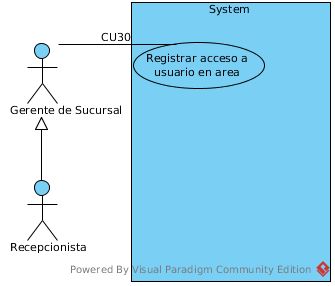
\includegraphics[width=0.4\textwidth]{images/CU30}
  		\caption{CU30 registro de un usuario a area}
		\end{figure}
	}
		\UCitem{Versión}{1.0}
		\UCitem{Actor}{Gerente de Sucursal}
		\UCitem{Propósito}{Registrar el acceso de los clientes a una area.}
		\UCitem{Entradas}{ identificador RFID de la targeta de cada cliente}
		\UCitem{Origen}{Teclado}
		\UCitem{Salidas}{mensaje: Acceso autorizado }
		\UCitem{Destino}{Pantalla}
		\UCitem{Precondiciones}{El Cliente debe tener al corriente su cuenta de pago de la membresia adquirida.}
		\UCitem{Postcondiciones}{El sistema digital agregara un usuario mas a la cuenta de acceso a clientes de esa area donde se ubuca el lector.}
		\UCitem{Errores}{Que se vaya la luz}
		\UCitem{Tipo}{Caso de uso primario}
		\UCitem{Observaciones}{Los clientes son responsables de su propio acceso, debe de presentar su targeta durante la estancia de cualquer area del gimnasio.}
		\UCitem{Autor}{Carrillo Mendoza Martín Alejandro.}
		\UCitem{Reviso}{Francisco García Enríquez.}	
	\end{UseCase}
	\newpage
	\begin{UCtrayectoria}{Principal}
	\UCpaso[\UCactor] Presenta su targeta con su numero de cliente unico \IUref{IU30.0}{Pantalla de Control de Acceso}\label{CU30.0Login} para su lectura del sistema.
		\UCpaso Válida que el actor se encuentre dado de alta en la base de datos del sistema. Se utiliza la regla \BRref{BR117}{Determinar si el usuario tiene acceso al sistema.} \Trayref{A}.
		\UCpaso Despliega la \IUref{IU30.1}{Pantalla de acceso autorizado al area} que permite la señal de acceso a los torniquetes, donde se liberan y puede acceder el cliente a el area.
	
	\UCpaso Verifica que tenga el pago corresponiente al mes de su membresia del cliente. \BRref{BR13}{Validar el pago de memebresia del cliente} \Trayref{B}.
		
		\UCpaso Almacena un registro mas a el area  en la base de datos.
		\UCpaso Muestra el \IUref{UI30.1}{Acceso autorizado.}\Trayref{C}.
		\UCpaso Regresa a la pantalla principal de acceso a area\IUref{IU9.1}{Pantalla de acceso a Recepcionista de Sucursal}.
\end{UCtrayectoria}

\begin{UCtrayectoriaA}{A}{El actor no introduce nombre de usuario (username) y contraseña (password) para poder ingresar al sistema.}
			\UCpaso Muestra el mensaje {\bf MSG30.0-}``Error: acceso no peermitido [{\em y/o}] ''.
			\UCpaso Regresa a la pantalla principal de acceso a areas de sucursal\IUref{IU30.1}{Pantalla de acceso a areas de Sucursal}.
		\end{UCtrayectoriaA}

			
%-------------------------------------- TERMINA descripción del caso de uso.